\documentclass[ignorenonframetext, hyperref=unicode]{beamer}



\usepackage{cmap}
%\usepackage[T2A]{fontenc}
\usepackage[utf8]{inputenc}
\usepackage[bulgarian]{babel}
\selectlanguage{bulgarian}

\usepackage{color}
\usepackage{graphicx}
\usepackage{listings}
\usepackage{rcsinfo}
\usepackage{pgf}
\usepackage{supertabular}
\usepackage{rotating}

\hypersetup{
	colorlinks=true,
	linkcolor=blue,
	filecolor=blue,
	urlcolor=blue,
	anchorcolor=blue,
	citecolor=blue
}

\lstset{language=C++, 
  numbers=left, 
  numberstyle=\tiny,
  stepnumber=1, 
  numbersep=3pt, 
  tabsize=2, 
  texcl,
  basicstyle=\ttfamily\small,
  identifierstyle=\ttfamily\small,
  keywordstyle=\sffamily\bfseries\small,
  extendedchars=true, inputencoding=utf8,
  backgroundcolor=\color[rgb]{1,1,0.845},
  escapeinside={/*@}{@*/}}

%\usepackage{algpseudocode}
%\usepackage[ruled]{algorithm}

\newcommand{\Cpp}{{\ttfamily\bfseries C++}}
\newcommand{\CC}{{\ttfamily\bfseries C}}

\definecolor{outputcolor}{rgb}{0.0,0.0,0.5}
\newcommand{\aout}[1]{\color{outputcolor}{\begin{verbatim}#1\end{verbatim}}}

% \usepackage[T2A]{fontenc}
% \usepackage[cp1251]{inputenc}
% \usepackage[bulgarian]{babel}
\selectlanguage{bulgarian}




\newcommand{\lubo}{%
\author[Л.~Чорбаджиев]{Любомир Чорбаджиев\inst{1} \\ 
{\ttfamily lchorbadjiev@elsys-bg.org}}
\institute[ELSYS] % (optional, but mostly needed)
{
\inst{1}%
Технологическо училище ``Електронни системи'' \\
Технически университет, София
}}

\newcommand{\osauthors}{%
\author{
	В.Кетипов\\ 
	\and
	Н.Димитров \\ 
	\and
	{Х.Стефанов \\
	{\ttfamily elsys.os.2014@gmail.com}}
}
\institute[ELSYS] % (optional, but mostly needed)
{
\inst{1}%
Технологическо училище ``Електронни системи'' \\
Технически университет, София
}}

\titlegraphic{\href{http://creativecommons.org/licenses/by-sa/3.0/}{
\includegraphics{../macros/cc.png}}}

\newcommand{\ie}{т.~е.\ }

\newcounter{probcounter}[section]
\newenvironment{prob}[1][]%
        {\smallskip%
         \noindent\refstepcounter{probcounter}%
          \textbf{\theprobcounter${}^{#1}$.}\ }%
   {\medskip}

\mode<article>
{

}

\mode<presentation>
{
  \usetheme[secheader=true]{Madrid}
  \usecolortheme{crane}
  \usefonttheme[onlylarge]{structurebold}
  \setbeamercovered{transparent}
}

\usepackage[unicode]{hyperref}

%%% Local Variables: 
%%% mode: latex
%%% TeX-master: t
%%% End: 



\title{Процеси}
\lubo
\date{\today}

\begin{document}

\frame{\maketitle}

\begin{frame}
\frametitle{Съдържание}
\tableofcontents %[hideallsubsections]
\end{frame}

%-------------------------------------------------------------------- SECTION -
\section{Въведение}


%---------------------------------------------------------------------- SLIDE -
\begin{frame}\frametitle{Въведение}
\begin{itemize}
\item Компютърната система се състои от набор от хардуерни ресурси.
\item Софтуерните приложения се разработват за да изпълнят някаква задача.
\item Неефективно е приложенията да се разработват директно за дадена хардуерна
платформа.
\item Операционната система предоставя удобен за използване, богат на
възможности и еднообразен интерфейс, който може да се използва от приложенията.
\item Операционната система предоставя еднообразно абстрактно представяне на
ресурсите, които могат да се използват от едно приложение.
\end{itemize}
\end{frame}

%-------------------------------------------------------------------- SECTION -
\section{Процес}

%---------------------------------------------------------------------- SLIDE -
\begin{frame}\frametitle{Изпълнение на приложения}
\begin{itemize}
\item Изпълнението на приложенията се управлява от операционната система.
\item Операционната система разпределя ресурсите между приложенията, които се
изпълняват.
\item Процесорът се превключва между приложенията, които се изпълняват.
\item Това позволява по-ефективно използване на процесора и входно/изходните
устройства.
\item Операционните системи изпълняват различни приложения:
\begin{itemize}
  \item Системите за пакетна обработка -- задания.
  \item Системите с времеделене -- потребителски програми или задачи.
\end{itemize}
\item Задание, задача, процес $<=>$ процес.
\end{itemize}
\end{frame}

%---------------------------------------------------------------------- SLIDE -
\begin{frame}\frametitle{Дефиниция за процес}
\begin{itemize}
\item Процесът е програма, която се изпълнява.
\item Инструкциите на програмата се изпълняват последователно.
\item Единица работа, която може да се изпълнява върху процесора.
\item Единица работа, която се характеризира с изпълнение на последователност от
инструкции, текущо състояние и множество от системни инструкции.
\item Операционната система управлява изпълнението на процесите:
\begin{itemize}
	\item Изпълнява няколко процеса за да подобри използването на процесора.
	\item Заделя ресурси, необходимо за изпълнението на процесите.
	\item Предоставя механизми за комуникация между процесите.
	\item Предоставя средства за създаване на процеси от потребителя.
\end{itemize}
\end{itemize}
\end{frame}

%---------------------------------------------------------------------- SLIDE -
\begin{frame}\frametitle{Контролен блок на процеса}
\begin{itemize}
\item Съдържа информацията, необходима на операционната система за управление на
процеса:
\begin{itemize}
  \item Идентификация на процеса.
  \item Състояние на процеса.
  \item Приоритет.
  \item Програмен брояч.
  \item Данни за контекста на процеса.
  \item Информация за управление на паметта.
  \item Информация за състоянието на входно/изходните операции.
\end{itemize}
\item Създава се и се управлява от операционната система.
\item Позволява на операционната система да поддържа много процеси.
\end{itemize}
\end{frame}


%-------------------------------------------------------------------- SECTION -
\section{Състояние на процеса}

%----------------------------------------------------------------- SUBSECTION -
\subsection{Модел на процеса с две състояния}

%---------------------------------------------------------------------- SLIDE -
\begin{frame}\frametitle{Модел на процеса с две състояния}
\begin{itemize}
\item Всеки процес може да бъде само в две състояния:
\begin{itemize}
  \item Изпълнява се.
  \item Не се изпълнява.
\end{itemize}
\end{itemize}
\begin{figure}[h]
\center
\scalebox{0.7}{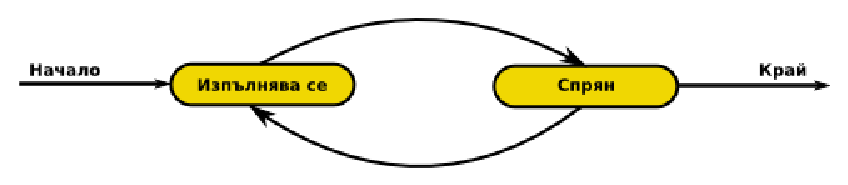
\includegraphics{pics/04-two-state-process-model}}
\end{figure}
\end{frame}

%---------------------------------------------------------------------- SLIDE -
\begin{frame}\frametitle{Модел на процеса с две състояния}
\begin{figure}[h]
\center
\scalebox{0.7}{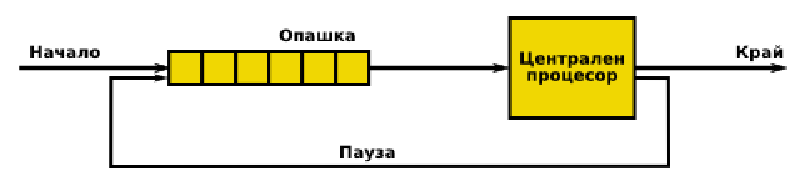
\includegraphics{pics/04-two-state-process-scheduling}}
\end{figure}
\begin{itemize}
\item Този модел е непълен. Може да има различни причини, поради които един
процес да бъде ``спрян'':
\begin{itemize}
  \item Готов за изпълнение.
  \item Блокиран върху входно/изходна операция.
\end{itemize}
\item Диспечера не може просто да избере процеса, който е първи в опашката,
защото този процес може да е блокиран.
\end{itemize}
\end{frame}

%----------------------------------------------------------------- SUBSECTION -
\subsection{Модел на процеса с пет състояния}


%---------------------------------------------------------------------- SLIDE -
\begin{frame}\frametitle{Модел на процеса с пет състояния}
\begin{itemize}
\item Нов -- създаване на процеса.
\item Изпълнява се -- инструкциите на процеса се изпълняват.
\item Блокиран -- процесът чака за някакво събитие (прекъсване от входно/изходна
операция).
\item Готов -- процесът е готов за работа и очаква да му бъде отпуснато
процесорно време.
\item Унищожен -- процесът е приключил изпълнението си.
\end{itemize}
\begin{figure}[h]
\center
\scalebox{0.7}{\includegraphics{pics/04-five-state-process-model}}
\end{figure}
\end{frame}

%---------------------------------------------------------------------- SLIDE -
\begin{frame}\frametitle{Модел на процеса с пет състояния}
\begin{figure}[h]
\center
\scalebox{0.9}{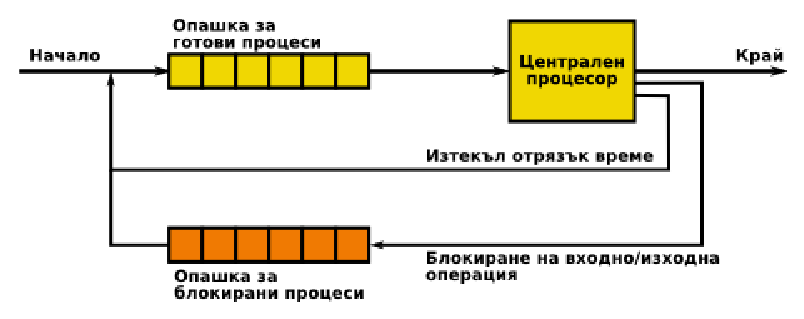
\includegraphics{pics/04-five-state-process-scheduling-2-queues}}
\end{figure}
\end{frame}

%----------------------------------------------------------------- SUBSECTION -
\subsection{Превключване на контекста}

%---------------------------------------------------------------------- SLIDE -
\begin{frame}\frametitle{Превключване на контекста}
\begin{itemize}
\item Когато процесорът се превключва от един към друг процес, операционната
система трябва да съхрани състоянието на предишния процес и да зареди запазеното
състояние на новия процес.
\item Превключването на контекста изисква време. Докато се превключва
контекста системата не може да изпълнява ``полезна'' работа.
\item Времето за превключване на контекста зависи от хардуерната поддръжка.
\end{itemize}
\end{frame}

%---------------------------------------------------------------------- SLIDE -
\begin{frame}\frametitle{Превключване на контекста}
\begin{figure}[h]
\center
\scalebox{0.32}{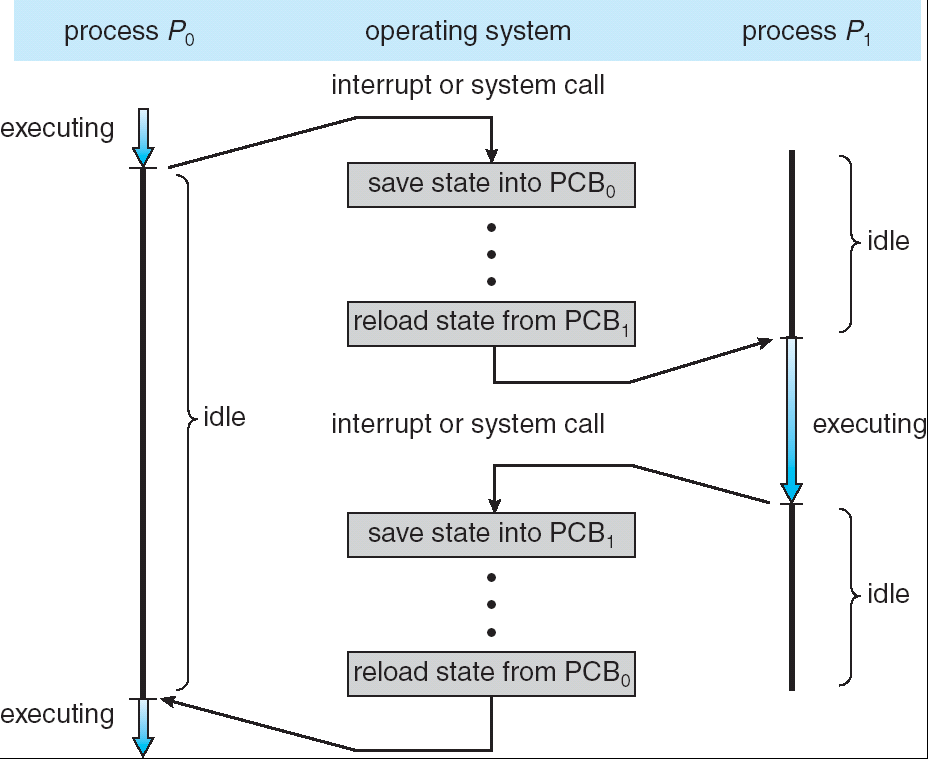
\includegraphics{pics/silberschatz7e-3-9-process-switch}}
\caption{Silberschatz, Gavin, Gagne: {\em Operating Systems Concepts}}
\end{figure}
\end{frame}

%---------------------------------------------------------------------- SLIDE -
\begin{frame}\frametitle{Превключване на контекста}
Има различни причини, които могат да доведат до превключване на контекста:
\begin{itemize}
\item Прекъсване от часовника -- процесът е работил максималният допустим
отрязък време.
\item Входно/изходно прекъсване.
\item Страница от паметта е във виртуалната памет и трябва да се качи в
оперативната памет.
\item Софтуерно прекъсване -- грешка при изпълнение на програмата. Може да доведе
до унищожаване на процеса.
\item Извикване на системна функция.
\end{itemize}
\end{frame}

%---------------------------------------------------------------------- SLIDE -
\begin{frame}\frametitle{Превключване на контекста}
\begin{itemize}
\item Съхраняване на контекста на процесора, включително програмния брояч и
другите регистри.
\item Обновяване на контролния блок на процеса и промяна на състоянието.
\item Преместване на контролния блок на процеса в някоя от опашките от процеси
--- опашката на готовите процеси, опашката на блокираните процеси и т.н.
\item Избиране на следващ процес за изпълнение.
\item Обновяване на контролния блок на избрания процес.
\item Възстановяване на контекста на избрания процес.
\end{itemize}
\end{frame}




%-------------------------------------------------------------------- SECTION -
\section{Създаване на процес}

%---------------------------------------------------------------------- SLIDE -
\begin{frame}\frametitle{Създаване на процес}
\begin{itemize}
\item Процесите са организирани в дървовидна структура. Родителският процес
създава процеси, които са негови деца. Децата на свой ред могат да създават
процеси, които са техни деца.
\item При създаването, процесът:
\begin{itemize}
  \item получава уникален идентификатор на процеса;
  \item заделя се пространство, необходимо за изпълнението на процеса;
  \item инициализира се контролния блок на процеса;
  \item контролния блок на процеса се добавя във всички необходими таблици,
  посредством които операционната система контролира работата на процеса.
\end{itemize}
\end{itemize}
\end{frame}

%---------------------------------------------------------------------- SLIDE -
\begin{frame}\frametitle{Създаване на процес: UNIX}
\begin{itemize}
\item В UNIX за създаване на процес се използва системната функция
\lstinline{fork()}.
\item Новосъздадения с \lstinline{fork()} процес представлява точно копие на
родителския процес.
\item Трябва да се използва някоя от фамилията системни функции
\lstinline{exec*()} за да се зареди в адресното пространство на процеса нова
програма.
\end{itemize}
\end{frame}


%---------------------------------------------------------------------- SLIDE -
\begin{frame}\frametitle{Унищожаване на процес}
\begin{itemize}
\item След като процесът изпълни последния си оператор, той се обръща към
операционната система за да я накара да го изтрие. Това се изпълнява със
системната функция \lstinline{exit()}.
\item При унищожаването на процеса, операционната система предава информация за
това към неговия родителски процес посредством системната функция
\lstinline{wait()}.
\item Ресурсите заемани от процеса се освобождават.
\item Родителският процес е в състояние да прекрати изпълнението на процесите,
които са му деца.
\item Когато родителският процес бъде прекратен, операционната система типично
унищожава и неговите деца.
\end{itemize}
\end{frame}

%---------------------------------------------------------------------- SLIDE -
\begin{frame}\frametitle{Създаване и унищожаване на процес: UNIX}
\begin{itemize}
\item 
\lstinline{pid_t fork (void)}
\item 
\lstinline{int execv (const char *filename, char *const argv[])}
\item 
\lstinline{int execl (const char *filename, const char *arg0, . . . )}
\item
\lstinline{pid_t waitpid (pid t pid, int *status, int options)}
\end{itemize}
\end{frame}


%---------------------------------------------------------------------- SLIDE -
\begin{frame}[containsverbatim]
\frametitle{Създаване на процес: UNIX}
\lstinputlisting[lastline=16]{code/fork01.cc}
\end{frame}

%---------------------------------------------------------------------- SLIDE -
\begin{frame}[containsverbatim]
\frametitle{Създаване на процес: UNIX}
\lstinputlisting[firstline=16,lastline=160]{code/fork01.cc}
\end{frame}

%---------------------------------------------------------------------- SLIDE -
\begin{frame}[containsverbatim]
\frametitle{Създаване на процес: UNIX}
\lstinputlisting[lastline=16]{code/fork02.cc}
\end{frame}

%---------------------------------------------------------------------- SLIDE -
\begin{frame}[containsverbatim]
\frametitle{Създаване на процес: UNIX}
\lstinputlisting[firstline=16,lastline=160]{code/fork02.cc}
\end{frame}


%---------------------------------------------------------------------- SLIDE -
\begin{frame}[containsverbatim]
\frametitle{Създаване на процес: UNIX}
\begin{verbatim}
lubo@baby ~/school/workspace/os04/code $ ./fork02 
going to run shell from child...
sh-3.2$ ls -l
total 24
-rwxr-xr-x 1 lubo wheel 7580 2007-10-23 12:15 fork01
-rw-r--r-- 1 lubo wheel  679 2007-10-23 12:22 fork01.cc
-rwxr-xr-x 1 lubo wheel 7581 2007-10-23 12:44 fork02
-rw-r--r-- 1 lubo wheel  648 2007-10-23 12:44 fork02.cc
sh-3.2$ exit
exit
child process finished 0...
\end{verbatim}
\end{frame}


%-------------------------------------------------------------------- SECTION -
\section{Сътрудничество между процеси}

%---------------------------------------------------------------------- SLIDE -
\begin{frame}\frametitle{Сътрудничество между процеси}
\begin{itemize}
\item Процесите са изолирани и по принцип те не могат да въздействат на
изпълнението на други процеси.
\item Сътрудничеството между процеси предполага наличието на механизми,
посредством които даден процес да може да въздейства върху изпълнението на друг
процес.
\item Сътрудничеството между процеси има ред предимства:
\begin{itemize}
  \item Увеличаване на производителността.
  \item Подобряване на модулността на приложенията.
  \item Удобство при разработка.
\end{itemize}
\end{itemize}
\end{frame}
       

\end{document}
